\documentclass{beamer}

\begin{filecontents}{ref.bib}
    @inproceedings{struhr,
    author =	{V{\'a}clav Struh{\'a}r and Moris Behnam and Mohammad Ashjaei and Alessandro V. Papadopoulos},
    title =	{{Real-Time Containers: A Survey}},
    booktitle =	{2nd Workshop on Fog Computing and the IoT (Fog-IoT 2020)},
    year =	{2020},
    }
    @inproceedings{barletta2022achieving,
    title={Achieving isolation in mixed-criticality industrial edge systems with real-time containers},
    author={Barletta, Marco and Cinque, Marcello and De Simone, Luigi and Della Corte, Raffaele},
    booktitle={34th Euromicro Conference on Real-Time Systems (ECRTS 2022)},
    year={2022},
    organization={Schloss Dagstuhl-Leibniz-Zentrum f{\"u}r Informatik}
    }
    @inproceedings{abranches2019shimmy,
    title={Shimmy: Shared memory channels for high performance inter-container communication},
    author={Abranches, Marcelo and Goodarzy, Sepideh},
    booktitle={USENIX Workshop on Hot Topics in Edge Computing (HotEdge)},
    year={2019}
    }
\end{filecontents}


\usepackage{wrapfig}
\usepackage{algpseudocode}
\usepackage{algorithm}

\usetheme{Boadilla}
\usecolortheme{dolphin}
\setbeamertemplate{navigation symbols}{}
\setbeamertemplate{sections/subsections in toc}[sections numbered]

\title{Real-time Containers Technology}
\author[MirSattarian, Afkar]{Sina MirSattarian \and Hossein Afkar}
\institute{University of Tehran}
\date{\today}

\begin{document}

\frame{\titlepage}

\begin{frame}
    \frametitle{Table of Contents}
    \tableofcontents[hideallsubsections]
\end{frame}

\section{Introduction: Real-time Containers Survey}
\begin{frame}
    \frametitle{Introduction}
    This survey was included in 2nd Workshop on Fog Computing and the IoT
    (Fog-IoT 2020) \cite{struhr} \\
    Cloud and Edge computing relies extensively on resource virtualization.
    The containter-based virtualization is gaining its importance as a
    lightweight alternative of hypervisor-based virtualizaion. Container based
    virtualization does not require a hypervisor and therefore it provides
    near-native performance.
\end{frame}

\begin{frame}
    \frametitle{Containerization Benefits for Real-time Community}
    Requirements of the companies that operate in areas such as industrial
    and robot control, automotive and aviations are:
    \begin{itemize}
        \item Consolidate computational resources (Electronic Control Units,
            physical controllers).
        \item Provide a flexible environment for running real-time applications.
        \item Enable interruption-free hardware and software maintainance.
        \item Dynamic system redundancy and system redundancy healing.
    \end{itemize}
\end{frame}

\begin{frame}
    \frametitle{Container-based Virtualization}
    Containers are a set of resource isolated process that are isolated from
    the rest of the system and other containers.
    This is achieved by using cgroups and namespaces.
\end{frame}

\begin{frame}
    \frametitle{Container Platfroms}
    \begin{itemize}
        \item LXC: The first user of cgroups and namespaces and pioneer of the
            containers on linux.
        \item Docker: Most popular solution for containerization.
    \end{itemize}
\end{frame}

\begin{frame}
    \frametitle{Real-time support in linux as the container host}
    Cgroups is a tightly coupled extension of the scheduler. The default
    scheduler of linux does not give any time guarantees on the execution of the
    procesess. There are several ways of implementing the real-time capability
    in the linux kernel.
\end{frame}

\begin{frame}
    \frametitle{Survey Results on Real-time Container Methods}
    \begin{itemize}
        \item PREEMPT\_RT Patch.
        \item Real-time Co-Kernel: In this method real-time co-kernel runs
            alongside the linux kernel and handles time critical activites
            like interrupt handling and scheduling real-time tasks and lets
            standard linux run when the co-kernel is idle. It requires special
            tools and apis for applications deployment. This modular architecture
            requires special care in the design. [RTAI and Xenomai]
        \item Hierarchical Scheduling of Containers: An example was designed by
            Cucinotta, Albeni et al, where the linux scheduler was modified
            to provide two levels of scheduling. The first level was an EDF
            scheduler that was used on the containers. The second level used a
            fixed priority scheduler to select a task in the container.
    \end{itemize}
\end{frame}

\begin{frame}
    \frametitle{Challenges}
    \begin{itemize}
        \item Lack of tools for real-time container management.
            [orchestration tool, Middleware that is aware of
            the communications and isolation needs]
        \item Communication between real-time containers.
            [Security and data management shared across the containers]
        \item Lack of Safety and security analysis tools.
        \item Lack of performance and latency test.
        \item Processes in the containers are not aware of a resource-limited
            isolated environment co-located with other containers.
    \end{itemize}
\end{frame}

\section{Achieving Isolation in Mixed-
Criticality Industrial Edge
Systems with Real-Time
Containers}
\begin{frame}
    \frametitle{Introduction}
    This paper was presented in ECRTS \cite{barletta2022achieving}
    \begin{itemize}
        \item Why Real-time containers?
        \item Why Isolation is very important
    \end{itemize}
\end{frame}

\begin{frame}
    \frametitle{Container-based Virtualization Characterisitcs}
    \begin{itemize}
        \item Low overhead
        \item Simplified migration/orchestration
        \item Increased scalability
    \end{itemize}
\end{frame}

\begin{frame}
    \frametitle{Proposal}
    \begin{itemize}
        \item Hierarchical scheduling solution
        \item Real-time co-kernel
        \item Schedulability test
        \item POSIX-compliant
        \item Real-time networking stack
    \end{itemize}
\end{frame}

\begin{frame}
    \frametitle{Architecture}
    \begin{figure}
        \centering
        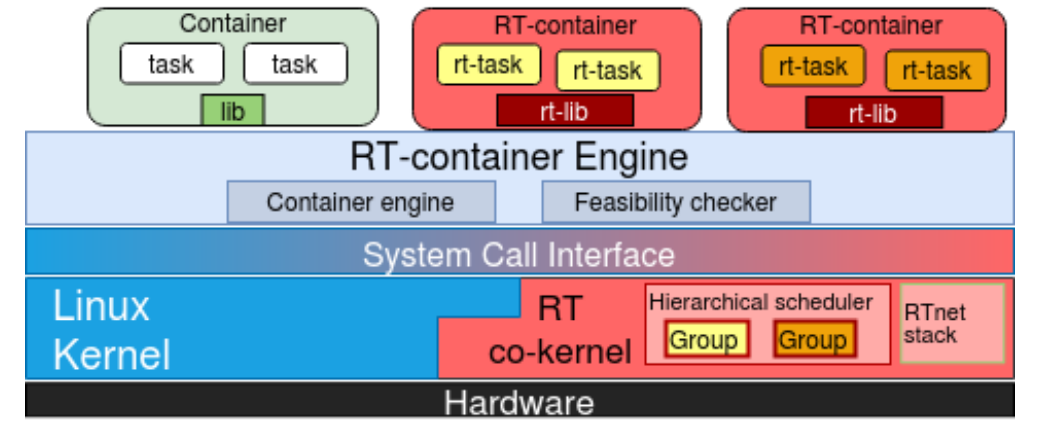
\includegraphics[width=1.0\textwidth]{mcs.png}
        \caption{The proposed rt-container architecture}
        \label{fig:mcs}
    \end{figure}
\end{frame}

\section{Shimmy: Memory Channels for High
    Performance Inter-Container Communication}
\begin{frame}
    \frametitle{Introduction}
    This paper was presented in usenix workshop \cite{abranches2019shimmy} \\
    The increased use of the reactive services and the need to process large
    amount of data has made the technologies like edge cloud to emerge. \\
    Applications are moving towards a microservice architectures, which means
    the applications are broke down into isolated small pieces. \\
    This isolation improves the deployability, but also introduces
    inefficiencies in communications. \\
    Approach used in this paper makes local and remote 
    communications more efficient.
\end{frame}

\begin{frame}
    \frametitle{Motivating Example}
    This paper provides us with a motivating example of a image processing
    pipeline
    \begin{figure}
        \centering
        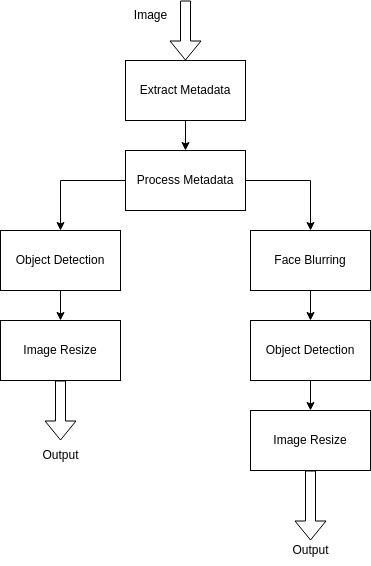
\includegraphics[width=0.4\textwidth]{pipeline.png}
        \label{fig:pipe}
    \end{figure}
\end{frame}

\begin{frame}
    \frametitle{Proposed Architecture}
    \begin{figure}
        \centering
        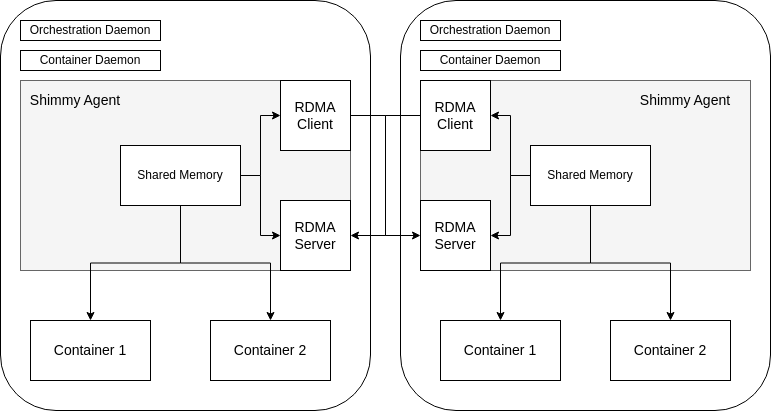
\includegraphics[width=1.0\textwidth]{arch.png}
        \caption{Systtem Architecture based on RDMA and shimmy agent}
        \label{fig:arch}
    \end{figure}
\end{frame}

\begin{frame}
    \frametitle{Establishing Shared Memory Channels}
    \begin{itemize}
        \item Allocating Memory: use shmget syscall
        \item Attaching to a container: docker has support for using the
            host shared memory space
        \item Application Interface: shm\_id should be passed to the
            application to be used with shmat syscall. An API must be provided.
        \item Communication across machines is done with RDMA. This technology
            copies the memory without the processor being involved.
    \end{itemize}
\end{frame}

\begin{frame}{Reference}
\bibliographystyle{apalike}
\bibliography{ref.bib} 
\end{frame}

\begin{frame}
  \centering \Large
  \emph{Thank You For Your Attention}
\end{frame}

\end{document}
